\documentclass[11pt]{beamer}
\usetheme{Darmstadt}
\useoutertheme{split}
\useoutertheme{miniframes}
\usepackage{hyperref}
\hypersetup{colorlinks, urlcolor=blue}
\usepackage{bm}
\usepackage{times}
\usefonttheme{structurebold}
\usepackage{array}
\usepackage[english]{babel}
\usepackage{amsmath,amssymb}
\usepackage[latin1]{inputenc}

%Code snippets and syntax highlighting
\usepackage{listings}
%Settings for Listings
\lstset{
  language=Python,
  basicstyle=\ttfamily,
  keywordstyle=\color{blue}\ttfamily,
  stringstyle=\color{red}\ttfamily,
  commentstyle=\color{green}\ttfamily,
  morecomment=[l][\color{magenta}]{\#}
}

\usepackage{array}
\usepackage{threeparttable}
\usepackage{colortbl}
\usepackage{multirow}
\usepackage{amsthm}
\usepackage{float,graphicx,color}
\newtheorem*{thm}{Theorem}
\theoremstyle{definition}
%\numberwithin{equation}{section}
\newtheorem*{defn}{Definition}
\newcommand\boldline{\arrayrulewidth{1pt}\hline}
\newcommand\ve{\varepsilon}


\setbeamercovered{dynamic}

\title[Short version of title]{Full version of title}
\author[FirstAuthor and SecondAuthor]{\textbf{First Author} \and \textbf{Second Author}}
\date{February 2019}


\begin{document}

\frame{\titlepage}


\section{Intro}  % This puts a section heading at the top of the slides

  \frame{
  \frametitle{Introduction}
    \begin{enumerate}
      \item<1-> This is a numbered list
      \item<2-> This second item in numbered list comes up on next click
      \vspace{5mm}
      \item<3-> The vspace command puts spaces between your items
    \end{enumerate}
    \begin{itemize}
      \item<4-> Bulleted lists are also good
      \item<4-> And you can set all the bullets to appear at once
    \end{itemize}
    \begin{block}<5->{Block (blue) and alertblock (red)}
      The block and alertblock environment makes these nice boxes that add emphasis
    \end{block}
  }


\section{Images}

  \begin{frame}
  \frametitle{Here is an image}
    \begin{figure}[htb]\centering
    \fbox{\resizebox{3.5in}{2.7in}{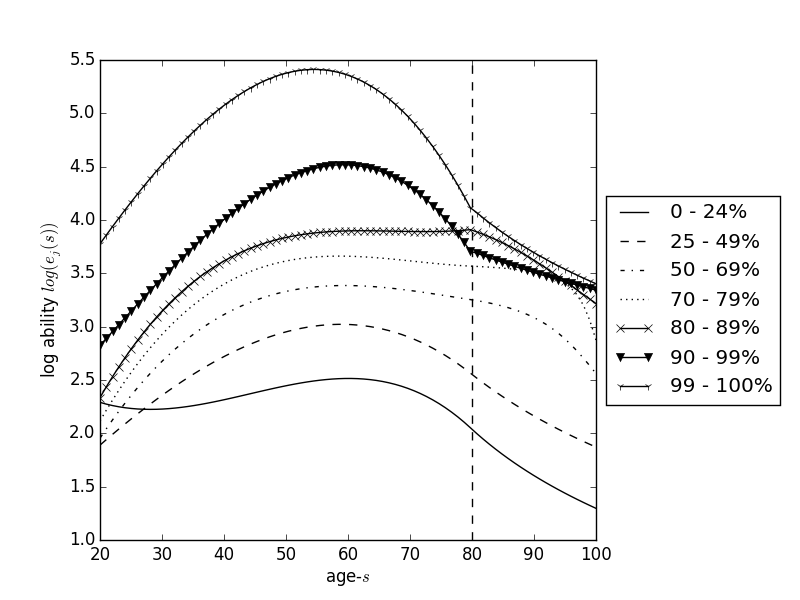
\includegraphics{images/ability_log_2D.png}}}
    \end{figure}
  \end{frame}


\section{Tables}

  \frame{
  \frametitle{Here is a table}
    \begin{tabular}{>{\small}c >{\small}l >{\small}r}
      \hline\hline
      Variable & Description & Value \\
      \hline
      $\beta$ & discount factor & 0.96 \\
      $\alpha$ & capital share of income & 0.35 \\
      \hline\hline
    \end{tabular}
  }


\end{document}
